\pdfoutput=1 %arXiv flag 

\documentclass[11pt]{article}
\usepackage{NotesTeX,lipsum}
%\usepackage{todonotes}
\usepackage{tikz,xcolor}
\usepackage{karnaugh-map}
\usepackage[utf8]{inputenc}
\usepackage[english]{babel}
\usepackage{amssymb,amsmath,amsfonts,amsthm}
\usepackage{verbatim}
\usepackage{enumerate}
\usepackage{tensor}
\usepackage{bbm}
\usepackage{graphicx}
\newlength{\xxxscale}
\setlength{\xxxscale}{0.065\textwidth}
\graphicspath{{apics/}}
\usepackage[caption=false]{subfig}



%%%%%%%%%%%%%%%%%%%%%%%%%%%%%%%%%%%%%%%%%%%%%%%%%%
%\usepackage{/Book-Tensor-Network/NotesTeX}



%%%%%%%%%%%%%%%%%%%%%%%%%%%%%%%%%%%%%%%%%%%
%\usepackage{natbib} % removed due to log error 

%\usepackage[hyperref=auto,style=numeric,defernumbers=true,backend=bibtex]{biblatex}
%\bibliography{qc.bib}
%\addbibresource{qc.bib}
%\ExecuteBibliographyOptions{firstinits=true,doi=false,sorting=none}
%\newbibmacro{string+doi}[1]{%
 %\iffieldundef{doi}{#1}{\href{http://dx.doi.org/\thefield{doi}}{#1}}}
%\DeclareFieldFormat{title}{\usebibmacro{string+doi}{\mkbibemph{#1}}}
%\DeclareFieldFormat[article]{title}{\usebibmacro{string+doi}{\mkbibquote{#1}}}

\newtheorem{observation}[theorem]{Observation}
%%%%%%%%%
\newcommand{\YX}{\mathcal{Y}\otimes\mathcal{X}}
\newcommand{\XY}{\mathcal{X}\otimes\mathcal{Y}}
\newcommand{\K}{{\mathbb K}}  % abstract field
\newcommand{\x}{\mathbf{x}}
\newcommand{\y}{\mathbf{y}}
\newcommand{\R}{{\mathbb R}}  % real numbers
\newcommand{\C}{{\mathbb C}}  % complex numbers
\newcommand{\hilb}[1]{\ensuremath{\mathcal{#1}}} % Hilbert space
%%%%%%%%%%%%%%%%%
\newcommand{\fscale}{1.0}
\newcommand{\incpdftex}[3][1.0]{\renewcommand{\fscale}{#1} \def\svgwidth{#2\textwidth} \input{apics/#3.pdf_tex}}
%%%%%%%%%%%%%%%%%%%
%%%%%%%%%%%%%%%%%%%%%%%%%%%%%%%%%%
\newtheoremstyle{No.}% name of the style to be used
{}% measure of space to leave above the theorem. E.g.: 3pt
{}% measure of space to leave below the theorem. E.g.: 3pt
{}% name of font to use in the body of the theorem
{}% measure of space to indent
{\bfseries}% name of head font
{}% punctuation between head and body
{ }% space after theorem head; " " = normal interword space
{\thmname{#1}\thmnumber{ #2}\thmnote{ (#3)}}
{
\theoremstyle{No.}
\newtheorem{illexample}[theorem]{Illustration}}
%%%%%%%%%%%%%%%%%%%%%%%%%%%%%%%%%%%%%%%%%%%
\newtheorem{corollary}[theorem]{Corollary}
\newtheorem{myexercise}[theorem]{Exercise}
%\newtheorem{illexample}[theorem]{Illustration}
%%%%%%%%%%%%%%%%%%%%%%%%%%%%%%%%%%%%%%%%%%%%%%%%%%%%%%%%%%%%%%
\tcolorboxenvironment{illexample}{colback=pink!20!white, enhanced jigsaw,
colframe=pink!75!black,
before skip=10pt,
after skip=10pt,
breakable}
%%%%%%%%%%%%%%%%%%%%%%%%%%%%%%%%%%%%%%%%%%%%%%%%%%%%%%%%%%%%%%%
\tcolorboxenvironment{myexercise}{colback=green!5!white, enhanced jigsaw,
colframe=green!75!black,
before skip=10pt,
after skip=10pt,
breakable,}  
%%%%%%%%%%%%%%%%%%%%%%%%%%%%%%%%%%%%%%%%%%%%%%%%%%%%%%%%%%%%%%%
\newenvironment{myfullpage}
    {\smallskip\noindent\begin{minipage}
    {\textwidth+\marginparwidth+\marginparsep}\smallskip\smallskip}
    {\end{minipage}\vspace{.1in}}
%%%%%%%%%%%%%%%%%%%%%%%%%%%%%%%%%%%%%%%%%%%%%%%%%%%

%%%%%%%%%%%%%%%%%%%%%
\usepackage{tcolorbox}
%%%%%%%%%%%%%%%%%%%%

\DeclareMathOperator{\Real}{Re}
\DeclareMathOperator{\Imag}{Im}
\DeclareMathOperator{\Span}{span}
\DeclareMathOperator{\diag}{diag}

\newcommand{\Lx}[1]{{L(\mathcal{#1})}}
% fonts 
\def\1#1{{\bf #1}}
\def\2#1{{\cal #1}}
\def\7#1{{\mathbb #1}}
\newcommand{\I}{\mathbbm{1}} 
% TODO abstract index notation vs. components, which is which?
\newcommand{\bydef}{\stackrel{\mathrm{def}}{=}}
\renewcommand{\baselinestretch}{1}  % cancels any possible double spacing
\newcommand{\dket}[1]{\mbox{$\left|\left.#1\right\rangle\!\right\rangle$}}
\newcommand{\dbra}[1]{\mbox{$\left\langle\!\left\langle #1\right.\right|$}}

%%%%%%%%%%%%%%%%%%%%%%%%
\newcommand{\dketdbra}[2]{\mbox{$|#1\rangle\!\rangle\!\!\langle\!\langle #2|$}}

\newcommand{\dbradket}[2]{\mbox{$\langle\!\langle #1|#2\rangle\!\rangle$}}
\newtheorem{proposition}[theorem]{Proposition}
%%%%%%%%%%%%%%%%%%%%%%%%
\def\3#1{{\sl #1}}
\newcommand{\Tx}[1]{{T(\mathcal{#1})}}
\newcommand{\Cx}[1]{{C(\mathcal{#1})}}
\newcommand{\XX}{\mathcal{X}\otimes\mathcal{X}}
\newcommand{\YY}{\mathcal{Y}\otimes\mathcal{Y}}
\newcommand{\LXY}{L(\mathcal{X}\otimes\mathcal{Y})}
\newcommand{\XZ}{\mathcal{X}\otimes\mathcal{Z}}
\newcommand{\gate}[1]{\ensuremath{\text{\sf #1}}}
\newcommand{\COPY}[0]{\gate{COPY}}
\newcommand{\swap}{\gate{SWAP}}
\newcommand{\SWAP}{\gate{SWAP}}
\newcommand{\W}{\gate{W}}
\newcommand{\ADD}{\gate{ADD}}
\newcommand{\CNOT}{\gate{CNOT}}
\newcommand{\NOT}{\gate{NOT}}
\newcommand{\CN}{\gate{CN}}
\newcommand{\XOR}{\gate{XOR}}
\newcommand{\OR}{\gate{OR}}
%\newcommand{\COPY}{\gate{COPY}}
\newcommand{\AND}{\gate{AND}}
\newcommand{\NAND}{\gate{NAND}}
\newcommand{\XNOR}{\gate{XNOR}}
\newcommand{\NOR}{\gate{NOR}}
\newcommand{\ANF}{\gate{ANF}}
\newcommand{\PPRM}{\gate{PPRM}}
\newcommand{\SAT}{\gate{SAT}}
\renewcommand{\H}{\gate{H}}
\renewcommand{\d}{\mathrm{d}}
\newcommand{\Z}{\sigma^z}
%\newcommand{\COPY}[1]{\gate{COPY}\ensuremath{_{#1}}}
\newcommand{\GHZ}{\gate{GHZ}}
\newcommand{\TNS}{{\gate{TNS}}}
\newcommand{\inprod}[2]{\ensuremath{\left\langle #1, #2 \right\rangle}}

\newcommand{\isom}{\cong}  % isomorphic to
\newcommand{\bv}{e}     % basis vector
\newcommand{\spidx}[3]{^{(#1)}{}\indices{^{#2}_{#3}}}
\newcommand{\Figref}[1]{Fig.~\ref{#1}}
\newcommand{\Eqref}[1]{Eq.~\eqref{#1}}
%\newcounter{number}

\newcommand{\be}{\begin{equation}}
\newcommand{\ee}{\end{equation}}
\newcommand{\cat}[1]{\ensuremath{\mathcal{#1}}}
\newcommand{\Hom}[2]{\text{hom}_{\cat{C}}(#1,#2)}
\newcommand{\hilbert}[1]{\ensuremath{\mathcal{#1}}}
\newcommand{\cupket}[1]{\ket{\cup}_{#1}}
\newcommand{\capbra}[1]{\bra{\cup}_{#1}}

\title{\begin{center}{{\Huge{\bf{Lectures on Quantum Tensor Networks}}}}\\
{\itshape a pathway to modern diagrammatic reasoning}
\end{center}}
%\author{\Large Jacob Biamonte{\let\thefootnote\relax\footnote{{Version current as of \today.}\\~\\I would be grateful if you email me regarding any typos, errors or omissions you discover.\\~\\ Preprint available at \href{http://arxiv.org/abs/1912.10049}{arXiv:1912.10049}}}
%}

%PS
\let\oldthefootnote\thefootnote
\author{\Large Jacob Biamonte{\let\thefootnote\relax
\footnote{{Version current as of \today.}\\~\\I would be grateful if you email me regarding any typos, errors or omissions you discover.\\~\\ Preprint available at \href{http://arxiv.org/abs/1912.10049}{arXiv:1912.10049}}}
}
\let\thefootnote\oldthefootnote
% end PS


\affiliation{ 
Deep Quantum Laboratory\\
Skolkovo Institute of Science and Technology\\
3 Nobel Street\\
Moscow Russia 143026\\ 

e-mail: \href{j.biamonte@skoltech.ru}{j.biamonte@skoltech.ru}\\
web: \href{http://quantum.skoltech.ru}{http://quantum.skoltech.ru}

\vspace{15 mm}

\begin{center}
%  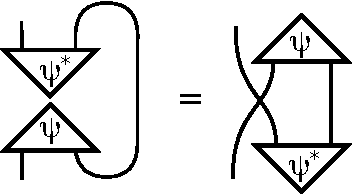
\includegraphics[width=0.5\textwidth]{penrose-density-state}
  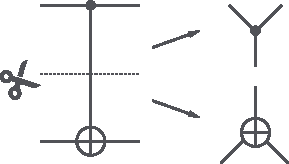
\includegraphics[width=0.5\textwidth]{cnot-tensors}
\end{center}
}

\begin{document}
	\maketitle
	%\flushbottom
	\newpage
	\pagestyle{fancynotes}
	\part*{Foreword}
Tensor network methods represent a collection of techniques to understand and reason about multi-linear maps which have found particular use in applications to quantum information processing.  These methods form the backbone of tensor network contraction algorithms to model physical systems and are used in the abstract graphical languages to represent channels, maps, states and processes appearing across quantum information science.  \\ 
	
In these chapters---which were complied based on years of teaching---we outline the  building blocks needed to understand the salient properties of tensor networks, the associated mathematical techniques and the diagrammatic reasoning language.   \\ 
	
The topic of tensor networks touches on a number of subjects yet the vast majority of writing is much more specific and often limited to be accessible by a narrow community. This book attempts to broadly cover the foundations of tensor network theory as it applies generally across quantum information.  \\ 
	
The aesthetically appealing development of tensor networks as a unifying language across quantum information science has long been close to my own research interests.  I have conducted research on quantum and classical circuits, as it applies to quantum computing.  This research included developing methods to embed logic functions into spin Hamiltonian ground states and the realization of quantum algorithms by quantum circuits.  The settings of both classical and quantum circuits comes with a well known graphical language.  \\

This provided a base to spend time merging ideas from (i) modern tensor networks as they appear in condensed matter physics; (ii) quantum circuits and their graphical language; (iii) aspects of categorical quantum mechanics as well as (iv) the graphical language of digital circuits to create a common notation and to develop and use rewrite rules that intersect these topics.  This book is intended to be self-contained, and accessible to graduate students.  It is hoped that advanced readers will let this book serve as a research reference.   \\
	
	
	Sincerely and happy reading, \\ 

~~~
\includegraphics[width=0.3\textwidth]{signature} \\  

Jacob Biamonte---Moscow \hfill \today 

\newpage 

\part*{Hall of Fame}
I humbly tip my hat to the following readers.  These brave souls found and reported typos, errors or omissions, improving the book for all future readers. \\ 

\noindent Konstantin Antipin \\
Nick Decroos \\ 
Sergey Filippov \\ 
Aly Nasrallah \\ 
Miles Stoudenmire \\ 
Alireza Yazdi 




\pagestyle{plain}


\include{chaps/Chapter1}  
 \include{chaps/Chapter2}
 \include{chaps/Chapter3}
 \include{chaps/Chapter4} 
 \include{chaps/Chapter-TNOQS}
 \include{chaps/Chapter5}
 
%  \section*{Afterword} 
%  Test. 


 \appendix
 \include{chaps/Appendix}

{    
    \bibliographystyle{unsrt}   
   \bibliography{qc.bib}
}

%  \bibliographystyle{unsrt}
%  \bibliography{qc}

% \printbibliography{}

\end{document}

